\documentclass[12pt]{article}

% Packages
\usepackage{graphicx}
\usepackage{amsmath}
\usepackage{geometry}
\geometry{margin=1in}
\usepackage{float}
\usepackage{caption}
\usepackage{subcaption}
\usepackage{cite}

\title{ME155C Final Project Report\\Inverted Pendulum Control: Swing-up, Balance, and Catching}
\author{Raaghav Thirumaligai, Cole Giusto, Tien Nguyen}
\date{June 8, 2025}

\begin{document}

\maketitle

\begin{abstract}
This project focuses on the identification, modeling, and control of an inverted pendulum on a cart system. Through experimental identification, control design, and closed-loop testing, we implemented robust swing-up, balancing, and catching controllers. System identification methods included logarithmic sine sweeps and parametric identification with MATLAB's tfest. Controller design employed energy-based swing-up methods and robust LQR/LQG balancing strategies. Experimental validations confirm effective performance, achieving stable equilibrium transitions and pendulum catching.
\end{abstract}

\section{Introduction}
This project investigates the control of an inverted pendulum on a cart, specifically targeting swing-up, balancing, and catching tasks. The inverted pendulum, a classic control problem, requires precise and robust feedback control strategies due to its inherent instability. Previous literature includes methods involving energy-based swing-up and state-space feedback stabilization. The report is structured with system identification in Section 2, controller design in Section 3, closed-loop results in Section 4, and conclusions in Section 5.

\section{System Identification}

\subsection{Process Description}
The experimental setup consists of an asymmetric metal rod mounted to a motor-driven cart, with encoders providing measurements of pendulum angle ($\theta$) and cart position ($x$). The control input is the motor voltage ($u$), and the primary controlled outputs are cart position and pendulum angle.

\begin{figure}[H]
    \centering
    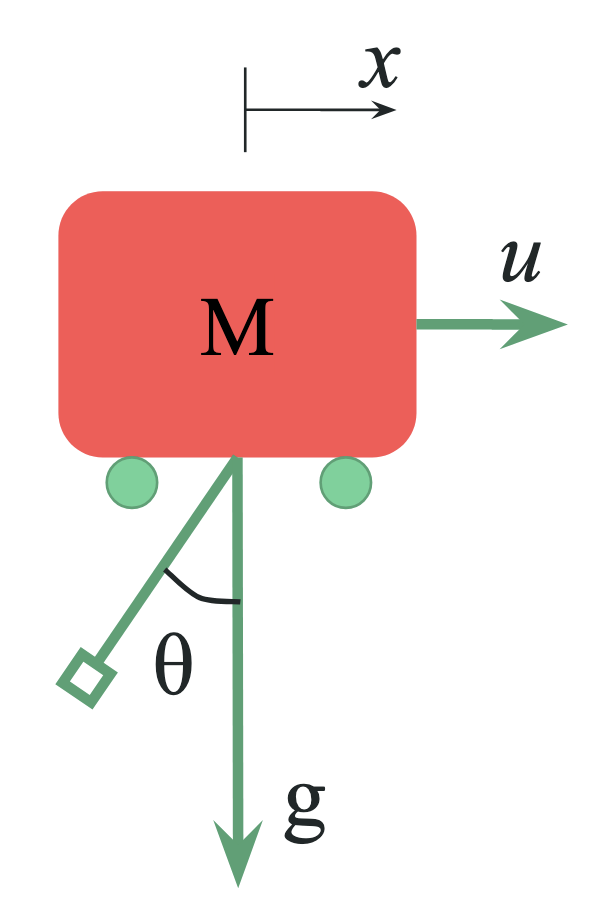
\includegraphics[width=0.15\textwidth]{figures/system_setup.png}
    \caption{Experimental setup: Cart-pendulum system.}
    \label{fig:setup}
\end{figure}

\subsection{Identification Methods}

Non-parametric identification utilized a logarithmic sine sweep ($0.3-3$ Hz). Parametric identification was done using MATLAB's \texttt{tfest} function, performing 30 experimental trials.

\begin{figure}[H]
    \centering
    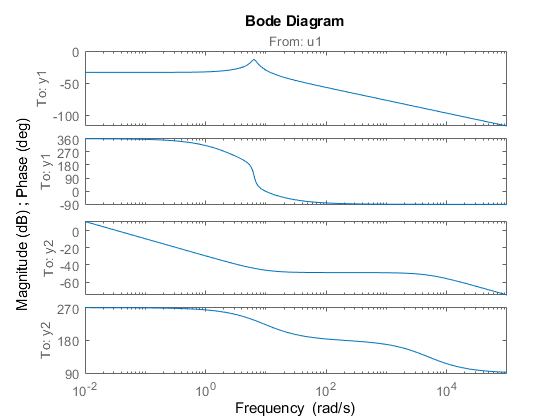
\includegraphics[width=0.8\textwidth]{../plots/bode_down.png}
    \caption{Bode plot: Identified frequency response for cart dynamics and pendulum dynamics downwards.}
    \label{fig:bode_down}
\end{figure}

\begin{figure}[H]
    \centering
    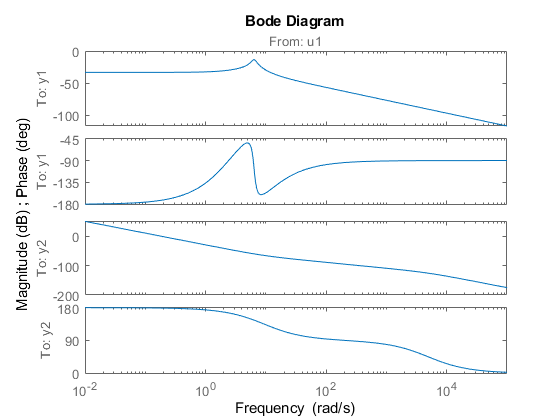
\includegraphics[width=0.8\textwidth]{../plots/bode_up.png}
    \caption{Bode plot: Identified frequency response for cart dynamics and pendulum dynamics upwards.}
    \label{fig:bode_up}
\end{figure}


\section{Controller Design}

\subsection{Swing-Up Controller}
An energy addition method drives the pendulum toward the upright position by strategically applying force near zero crossings of $\theta$, boosting the system's mechanical energy.

\begin{figure}[H]
    \centering
    
\includegraphics[width=0.6\textwidth]{figures/ph.png}
    \caption{Swing-up controller activation.}
    \label{fig:swingup}
\end{figure}

\subsection{Balancing Controller}
The balancing controller employs LQR/LQG methods to stabilize the pendulum in the inverted (unstable) equilibrium within a narrow angular region.

\subsection{Catching Controller}
Similar to balancing, catching employs LQR/LQG but aims to return the pendulum reliably to the stable downward equilibrium.

\subsection{State Machine}
Control modes transition between swing-up, balancing, and catching using a robust state machine architecture.

\begin{figure}[H]
    \centering
    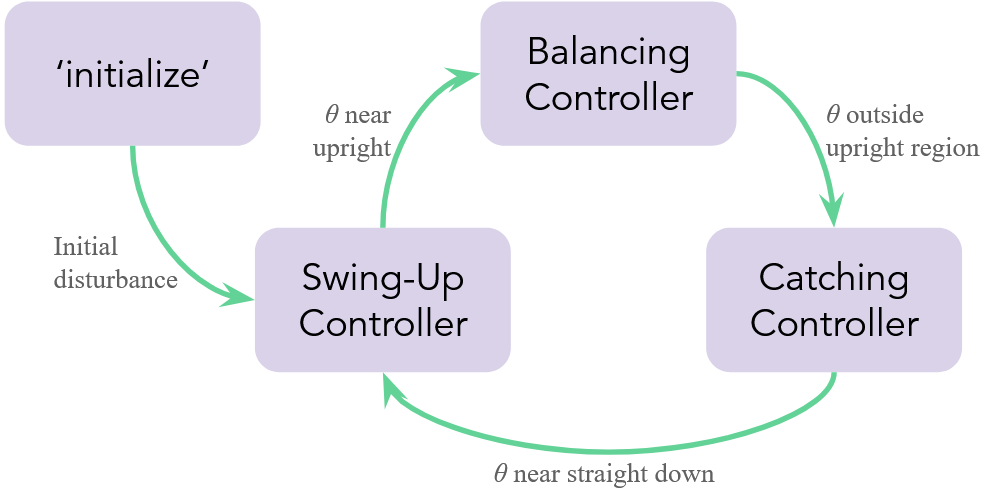
\includegraphics[width=0.6\textwidth]{figures/state_machine.png}
    \caption{State machine for mode switching between controllers.}
    \label{fig:state_machine}
\end{figure}

\section{Closed-Loop Performance}

Closed-loop experiments validated the controllers' performance. The step response showed quick stabilization and effective handling of mode transitions.

\begin{figure}[H]
    \centering
    
\includegraphics[width=0.8\textwidth]{figures/ph.png}
    \caption{Closed-loop step response for cart and pendulum positions.}
    \label{fig:step_response}
\end{figure}

\section{Conclusions and Future Work}
The controllers successfully addressed swing-up, balancing, and catching objectives, validating theoretical designs with robust experimental performance. Further work includes enhancing failure logic and addressing steady-state error.

\bibliographystyle{IEEEtran}
\bibliography{references}

\end{document}
